% ============================================================
% Motivation: multi-domain data, hard vs. soft interventions, CRISPRa
% ============================================================

\begin{frame}{Breaking the i.i.d. Assumption}
  \vspace{2ex}
  \begin{itemize}
    \item \textbf{Last Week --- Multi-View (MRI, CT, X-Ray):} Identically distributed across units, \emph{not} independent across views (shared $U$):
      \[
        (X_1,\dots,X_K) = (f_1(U),\dots,f_K(U)), \qquad
        \PP(X_1,\dots,X_K) \neq \prod_{k=1}^K \PP(X_k)
      \]
    \item \textbf{Today --- Multi-Domain (Interventions):} Independent across samples, \emph{not} identically distributed across domains:
      \[
        \cD \sim \PP_{f(U)}, \qquad \cD^{I_k} \sim \PP_{f(U^{I_k})}, \qquad k = 1,\dots,K
      \]
  \end{itemize}
  \sep
  \lbl{Why Multi-Domain?} Destructive measurements (CRISPR) prevent paired observations of the same unit across interventions.
\end{frame}

% ------------------------------------------------------------
\begin{frame}{Hard vs.\ Soft Interventions}
  \vspace{1ex}
  \centering
  \begin{tikzpicture}[x=1cm,y=1cm]
    % one panel: #1 x-offset
    \foreach \x/\name/\sub in {0/Observational/, 4.7/Hard/ (perfect), 9.4/Soft/ (imperfect)} {
      \node[font=\small] at (\x,1.65) {\textbf{\name}\sub};
    }
    % --- observational
    \node[var] (a1) at (0,1)    {$U_1$};
    \node[var] (a2) at (-0.95,-0.25) {$U_2$};
    \node[var] (a3) at (0.95,-0.25)  {$U_3$};
    \draw[edge] (a1) -- (a2); \draw[edge] (a1) -- (a3); \draw[edge] (a2) -- (a3);
    \node[font=\small] at (0,-0.95) {$U_2 = s_2(U_1,Z_2)$};
    \node[font=\scriptsize] at (0,-1.35) {normal mechanism};
    % --- hard
    \begin{scope}[xshift=4.7cm]
      \node[var] (b1) at (0,1)    {$U_1$};
      \node[var,fill=ethorange!45] (b2) at (-0.95,-0.25) {$U_2$};
      \node[var] (b3) at (0.95,-0.25)  {$U_3$};
      \draw[cut] (b1) -- (b2) node[midway,left=1pt,text=black,font=\small] {$\times$};
      \draw[edge] (b1) -- (b3); \draw[edge] (b2) -- (b3);
      \node[text=ethorange] at (-1.45,-0.05) {\Lightning};
      \node[font=\small] at (0,-0.95) {$U_2 = \tilde Z_2$};
      \node[font=\scriptsize] at (0,-1.35) {edge $1 \to 2$ \textbf{removed}};
    \end{scope}
    % --- soft
    \begin{scope}[xshift=9.4cm]
      \node[var] (c1) at (0,1)    {$U_1$};
      \node[var,fill=ethlightblue] (c2) at (-0.95,-0.25) {$U_2$};
      \node[var] (c3) at (0.95,-0.25)  {$U_3$};
      \draw[edge] (c1) -- (c2); \draw[edge] (c1) -- (c3); \draw[edge] (c2) -- (c3);
      \node[text=ethorange] at (-1.45,-0.05) {\Lightning};
      \node[font=\small] at (0,-0.95) {$U_2 = s_2^I(U_1,Z_2)$};
      \node[font=\scriptsize] at (0,-1.35) {\textbf{mechanism changed}, edge kept};
    \end{scope}
  \end{tikzpicture}
  \sep
  \centering\small
  \textbf{Hard:} we \textbf{set} $U_2$ --- its parents no longer matter. \qquad
  \textbf{Soft:} we only \textbf{nudge} $U_2$ --- its parents still act.

  \note{
    ~1.5 min
    \begin{itemize}
      \item Same 3-variable causal graph in all three panels; we intervene on $U_2$.
      \item Hard (perfect, do-) intervention: we set $U_2$ ourselves, e.g.\ $U_2 :=$ value or fresh independent noise. $U_2$ no longer listens to its parent $U_1$, so the edge $1\to2$ is cut. The graph changes.
      \item Soft (imperfect) intervention: we only change the mechanism that produces $U_2$ (e.g.\ add a shift). $U_1$ still influences $U_2$, the edge stays; only $\PP(U_2 \mid U_1)$ changes.
      \item Hard interventions are a special case of soft ones, so soft interventions are the weaker (more realistic) assumption, but they give us less information: we never see $U_2$ ``disconnected'' from its parents.
      \item This is exactly the setting of the paper: one soft intervention per latent node.
    \end{itemize}
  }
\end{frame}

% ------------------------------------------------------------
\begin{frame}{Example: CRISPR Activation (CRISPRa)}
  \vspace{1ex}
  \begin{columns}[T]
    \begin{column}{0.4\textwidth}
      \begin{itemize}
        \item CRISPRa \textbf{boosts} transcription of a chosen gene
        \item its regulators (parents) \textbf{still act} on it
        \item we can \textbf{shift} its expression, not \textbf{set} it to a value
      \end{itemize}
      \vspace{3ex}
      \[ U_i^I = s_i(U_{\pa(i)}, Z_i) + a \]
      \vspace{-1ex}
      {\small\textbf{soft (shift) intervention}}
    \end{column}
    \begin{column}{0.56\textwidth}
      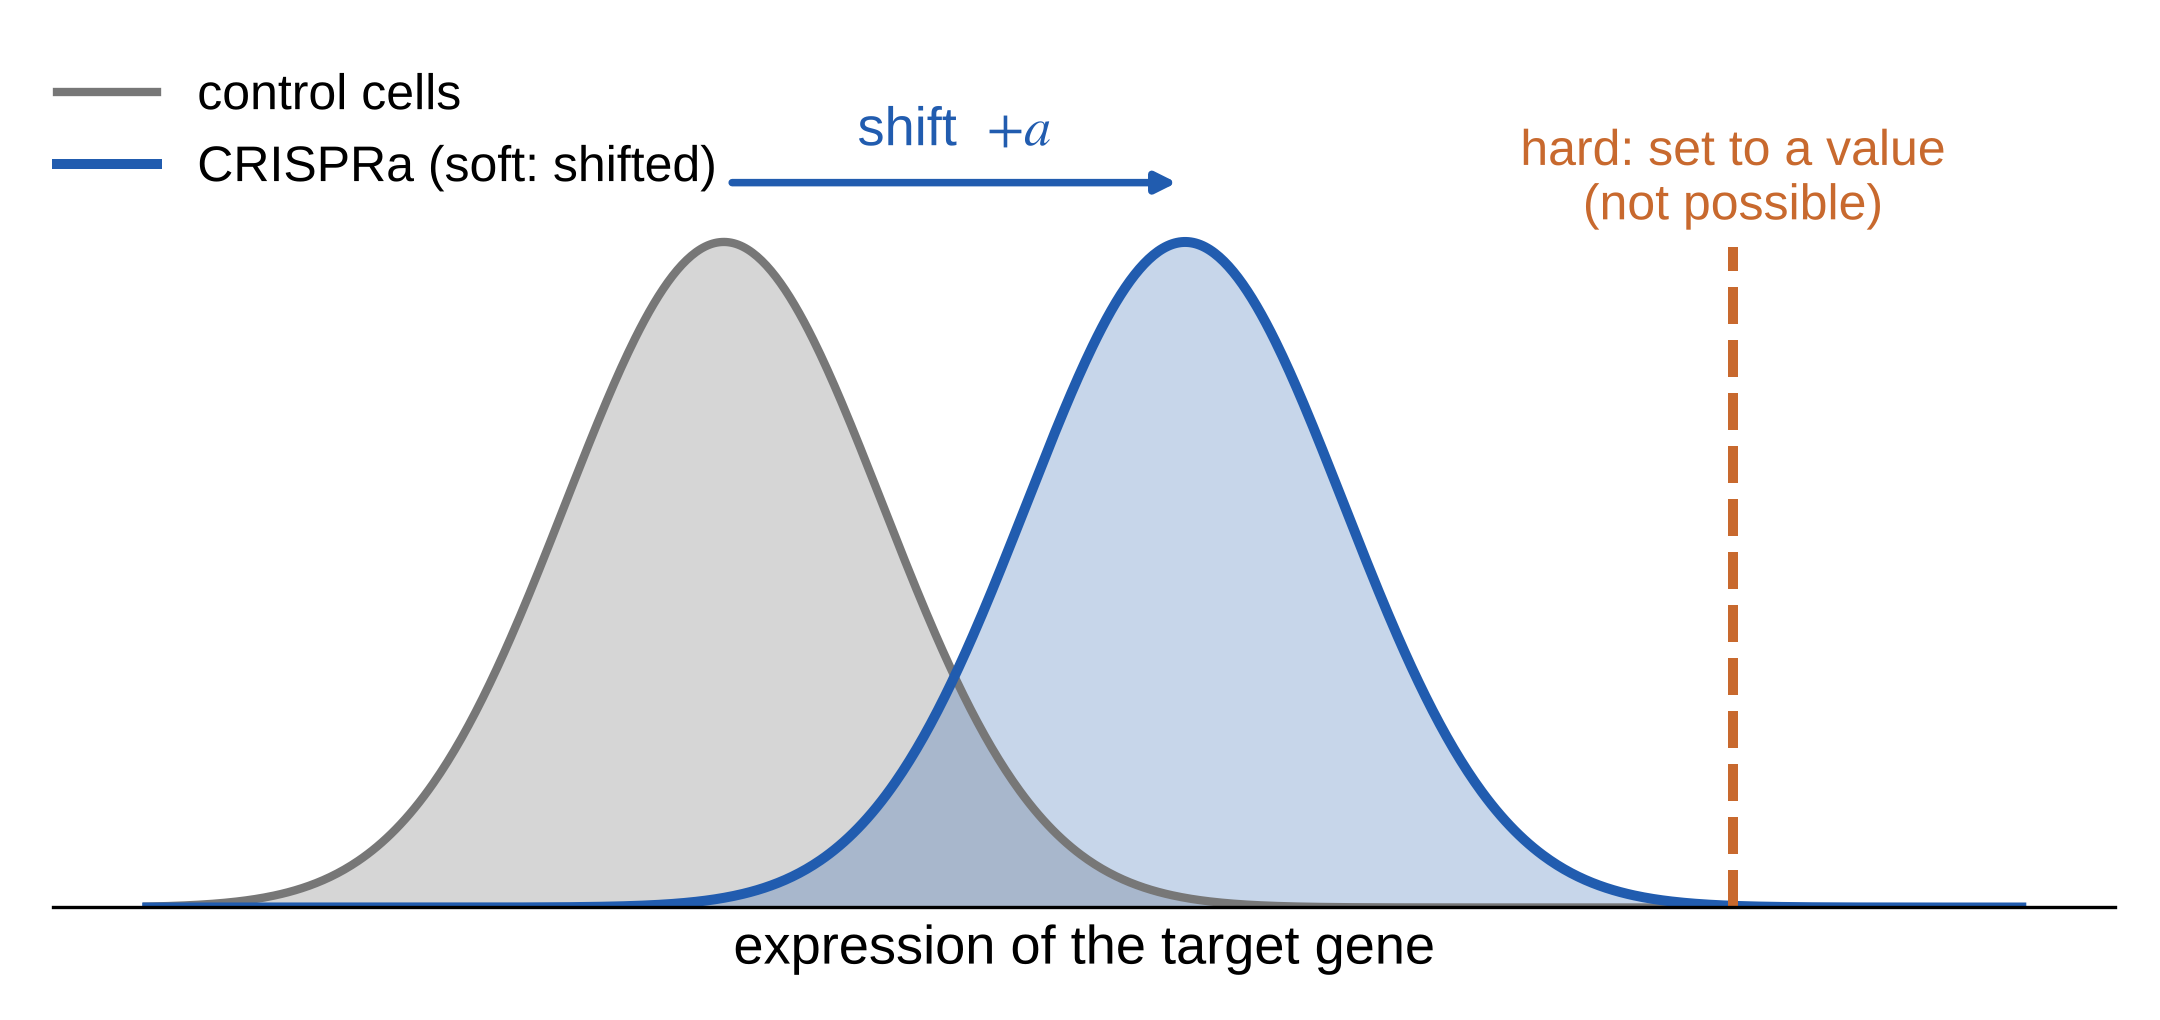
\includegraphics[width=\linewidth]{crispr_shift}
    \end{column}
  \end{columns}

  \note{
    ~1 min
    \begin{itemize}
      \item CRISPRa: a guide RNA brings a transcriptional activator to the promoter of a chosen gene, so the cell transcribes more of it.
      \item The gene's regulators (upstream transcription factors, i.e.\ its parents in the causal graph) keep acting on it: the expression level still varies from cell to cell and depends on the cell's state.
      \item So we can shift the expression up, but we cannot clamp it to a value of our choice: no hard intervention is available. In the model this is a shift intervention, $U_i \to s_i(U_{\pa(i)}, Z_i) + a$.
      \item This is the data used at the end of the talk (Perturb-seq, Norman et al.\ 2019).
    \end{itemize}
  }
\end{frame}
